\documentclass[11pt,a4paper]{article}
\usepackage[utf8]{inputenc}
\usepackage{mathtools}
\usepackage[norsk]{babel}
\usepackage{graphicx}
\usepackage{setspace}
\usepackage{tikz}
\usepackage{amsthm}
\usepgflibrary{shapes}
\usetikzlibrary{arrows,automata}
\usetikzlibrary{trees}


\usepackage{epstopdf}
 
\usepackage{color}
\definecolor{Blue}{rgb}{0.3,0.3,0.9}
\definecolor{Red}{rgb}{0.9,0.3,0.3}
\definecolor{Green}{rgb}{0.3,0.9,0.3}
\definecolor{ared}{rgb}{.647,.129,.149}

\usepackage{xcolor}

\newcommand\DrawCircleIns[2]{%
circle ({#2*cos(180/#1)})
}

\newtheoremstyle{mytheoremstyle} 	% name
    {\topsep}                    				% Space above
    {\topsep}                    				% Space below
    {\itshape}                   				% Body font
    {}                           					% Indent amount
    {\scshape}                   				% Theorem head font
    {.}                          					% Punctuation after theorem head
    {.5em}                       				% Space after theorem head
    {} 				 				% Theorem head spec (can be left empty, meaning ‘normal’)

\title{Notater: INF2080}
\author{Veronika Heimsbakk \\ 
veronahe@student.matnat.uio.no}
\begin{document}

\maketitle{}
\tableofcontents
\newpage{}

\section{Intro}
INF2080 - Logikk og Beregninger tar jeg våren 2013. Notatene er basert delvis på pensumboka (Sipser), egne forelesningsnotater, gruppeundervisning og foiler på kurssiden. Under semesteret oppdateres disse notatene når jeg gidder. Hovedsakelig i bruk for eksamensrepetisjon. Om noen ønsker \LaTeX markup som er brukt i notatene, er det bare å sende meg en e-post.

\section{Terminologi}
\subsection{Mengder}
En mengde er en endelig eller uendelig samling av objekter der rekkefølgen ignoreres. Objektene i en mengde kalles elementer.

\paragraph{Notasjon} $A = \{a, b, c\}, B = \{d, a, e\}$, den tomme mengden = $\emptyset$
\begin{itemize}
\item{I: a $\in$ \{a, b, c\}}
\item{Ikke i: d $\notin$ \{a, b, c\}}
\item{Delmengde: \{a\} $\subseteq$ \{a, b, c\}}
\item{Union: A $\cup$ B = \{a, b, c, d, e\}}
\item{Snitt: A $\cap$ B = \{a\}}
\item{Differanse: A / B = \{b, c\}}
\end{itemize}

\subsection{Boolsk logikk}
\begin{center}
\begin{tabular}{c c | c c c c c c}
& & og & eller & ikke & xor & ekvivalens & implikasjon\\
& & $\vee$ & $\wedge$ & $\neg$ & $\oplus$ & $\leftrightarrow$ & $\rightarrow$\\
\hline
0 & 0 & 0 & 0 & 1 & 0 & 1 & 1\\
0 & 1 & 0 & 1 & 0 & 1 & 0 & 1\\
1 & 0 & 0 & 1 & & 1 & 0 & 0\\
1 & 1 & 1 & 1 & & 0 & 1 & 1\\
\end{tabular}
\end{center}

\subsection{Nyttige definisjoner}
\begin{description}
\item[Symmetri] En binær relasjon R på mengden S er \textit{symmetrisk} hvis det for alle $x$, $y$ er slik at hvis $\langle x, y \rangle \in$ R, så $\langle y, x \rangle \in$ R.
\item[Refleksiv] En binær relasjon R på mengden S er \textit{refleksiv} hvis det for alle $x$ i S er slik at $\langle x, x \rangle \in$ R.
\item[Transitiv] En binær relasjon R på mengden S er \textit{transitiv} hvis det for alle $x$, $y$, $z$ er slik at hvis $\langle x, y \rangle \in $ R og $\langle y, z \rangle \in $ R, så $\langle x, z \rangle \in$ R.
\item[Ekvivalensrealsjon] En binær relasjon på mengden S er en \textit{ekvivalensrelasjon} hvis den er refleksiv, symmetrisk og transitiv.
\item[Injektiv] En funksjon $f : A \rightarrow B$ er \textit{injektiv} hvis for alle $x, y \in A$ så impliserer $x \neq y$ at $f(x) \neq f(y)$. Sier at $f$ er en-til-en.
\item[Surjektiv] En funksjon $f : A \rightarrow B$ er \textit{surjetiv} hvis for alle $y \in B$ så fins $x \in A$ slik at $f(x) = y$. Vi sier at $f$ er på.
\item[Bijektiv] En funksjon er \textit{bijektiv} hvis den er injektiv og surjektiv. Vi sier også at funksjonen er en en-til-en korrespondanse.
\item[Oppfyllbarhet] 
\item[Tautologi]
\item[Falisifiserbarhet] 
\item[Kontradiksjon]
\end{description}
\subsection{Grafer}
 \begin{figure}[h!]
 \centering
 \scalebox{0.7}
 {
 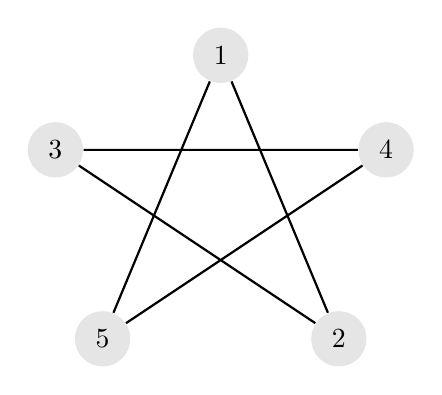
\begin{tikzpicture}[scale=6]
	 \tikzstyle{vertex}=[circle,minimum size=20pt,inner sep=0pt,fill=black!10]
	 \tikzstyle{selected vertex} = [vertex, fill=red!24]
	 \tikzstyle{selected edge} = [draw,line width=2pt,-,red!100]
	 \tikzstyle{edge} = [draw,thick,-,black]

	 \node[vertex] (v0) at (1,1.1) 		{5};
	 \node[vertex] (v1) at (1.5,1.1) 	{2};
	 \node[vertex] (v2) at (1.25,1.7) 	{1};
	 \node[vertex] (v3) at (1.6,1.5) 	{4};
	 \node[vertex] (v4) at (0.9,1.5) 	{3};

	 \draw[edge] (v0)  -- (v3) -- (v4) -- (v1) -- (v2) -- (v0); 
 \end{tikzpicture}
 }
 \caption{Eksempel på graf.}
 \end{figure}

En \textbf{urettet graf}, er en mengde linjer som kobler sammen noen punkter. Punktene kalles \textbf{noder} og linjene kalles \textbf{kanter}. Antall kanter til en node kalles \textbf{graden} til den noden. I Fig. 1 har alle nodene grad 2. 
 \begin{figure}[h!]
 \centering
 \scalebox{0.7}
 {
 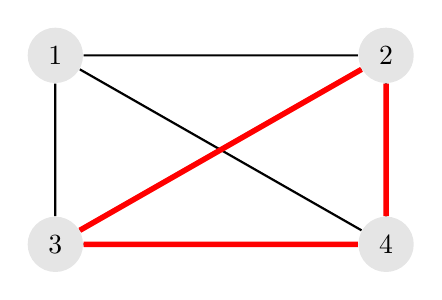
\begin{tikzpicture}[scale=6]
	 \tikzstyle{vertex}=[circle,minimum size=20pt,inner sep=0pt,fill=black!10]
	 \tikzstyle{selected edge} = [draw,line width=2pt,-,red!100]
	 \tikzstyle{edge} = [draw,thick,-,black, every path/.style={->}]
	 
	\node [vertex] (v0) at (0.5,0.5) 	{1};
	 \node[vertex] (v1) at (1.2,0.5) 	{2};
	 \node[vertex] (v2) at (0.5,0.1) 	{3};
	 \node[vertex] (v3) at (1.2,0.1) 	{4};

	\draw[edge] (v0)  -- (v1) -- (v3) -- (v2) -- (v0); 
	\draw[edge] (v0)  -- (v3) -- (v1) -- (v2); 
	\draw[selected edge] (v3) -- (v1) -- (v2) -- (v3);
 \end{tikzpicture}
 }
 \caption{Eksempel på graf med subgraf.}
 \end{figure}

I Fig. 2 er den rød streken en \textbf{subgraf} av hele grafen i figuren. De røde kantene representere også en \textbf{sti} gjennom grafen. En sti er en vei over kantene i en graf. En \textbf{rettet graf} er en graf med piler på kantene.


\subsection{Språk og alfabeter}


\section{Automater}
\subsection{Deterministiske}
\begin{figure}[h!]
\centering
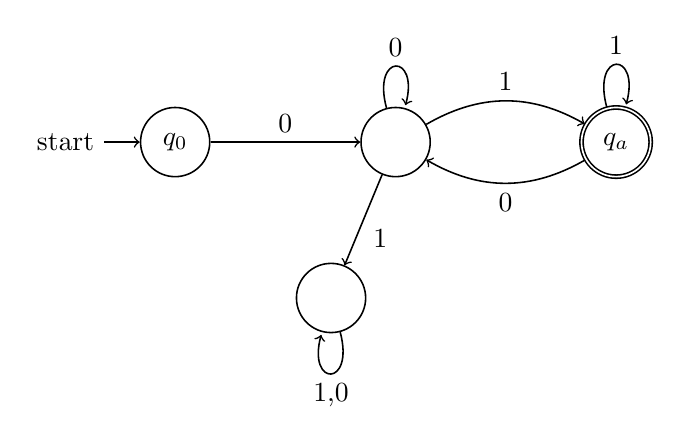
\begin{tikzpicture}[->,auto,node distance=2.8cm,line width=0.2mm]
  \node[initial,state] 	(A)                 	   			{$q_0$};
  \node[state]         		(B) [right of=A] 			{};
  \node[state]			(C) [below right of=A] 		{};
  \node[state,accepting]			(D) [right of=B] 	{$q_a$};

  \path 	(A) 	edge  node 				{0} 	(B)
        		(B) 	edge [loop above] node 	{0} 	(B)
			edge [bend left] node 		{1} 	(D)
			edge node 				{1} 	(C)
		(C) 	edge [loop below] node 	{1,0} (C)
		(D) 	edge [loop above] node 	{1} 	(D)
			edge [bend left] node 		{0} 	(B);
\end{tikzpicture}
\caption{Eksempel på en deterministic finite automata (DFA).}
\label{fig:dfa}
\end{figure}

\begin{itemize}
\item{Tilstander: 
\begin{tikzpicture}
  \draw[solid] (10,0) circle (0.3cm);
\end{tikzpicture}} 
, automaten over har fire tilstander. En automat består av én eller flere tilstander.
\item{Starttilstand: en automat har nøyaktig en starttilstand $q_0$.}
\item{Overganger: $\longrightarrow$, disse er markert med elementer fra alfabetet $\Sigma$= \{0,1\} (i eksempelet).}
\item{Akseptert tilstand: 
\begin{tikzpicture}
  \draw[solid] (10,0) circle (0.3cm);
	\draw (10,0) \DrawCircleIns{0.2}{0.2};
\end{tikzpicture}, det er x-antall slike aksepterte tilstander.}
\end{itemize}

\paragraph{Eksempel på input og utfall} for automaten i Figur ~\ref{fig:dfa}.
\begin{center}
\begin{tabular}{ l l }
	Input & Utfall\\
	\hline
	01 & akseptert\\
	010 & avvist\\
	0011 & akseptert\\
	00110 & avvist\\
\end{tabular}
\end{center}

La automaten i Figur ~\ref{fig:dfa} hete $M$, $M$ kjenner igjen språket: $L(M) = \{w |$  $w$ starter med $0$ og slutter med $1\}$. $L(M)$ er språket med en samling stringer $w$ som $M$ aksepterer. Eksempel: $0101$ er et element i $L(M)$, $0101 \in L(M)$.

\theoremstyle{mytheoremstyle}
\newtheorem{dfa}{Definisjon}[section]
\begin{dfa}
En \textbf{deterministic finite automata} er et 5-tuppel $(Q, \Sigma, \delta, q_0, F)$, hvor:

\begin{itemize}
	\item{$Q$ er et sett tilstander.}
	\item{$\Sigma$ er input alfabetet.}
	\item{$\delta$: $Q  \times \Sigma \rightarrow Q$ er pilenes funksjon.}
	\item{$q_0$ er $Q$ som starttilstand.}
	\item{$F \subseteq Q$ er de x-antall aksepterte.}
\end{itemize}
\end{dfa}

\paragraph{Eksempel}
Over språket $\Sigma = \{a,b\}$

\begin{figure}[h!]
\centering
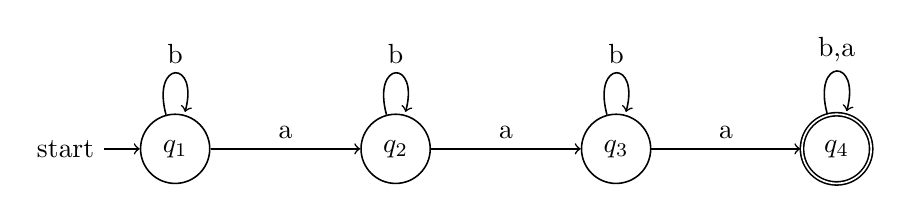
\begin{tikzpicture}[->,auto,node distance=2.8cm,line width=0.2mm]
  \node[initial,state] 			(A)		                 	{$q_1$};
  \node[state]         				(B) [right of=A] 	{$q_2$};
  \node[state]					(C) [right of=B] 	{$q_3$};
  \node[state,accepting]			(D) [right of=C] 	{$q_4$};

  \path 	(A) edge [loop above] node 		{b} 	(A)
			edge node 				{a} 	(B)
        		(B) edge [loop above] node 		{b} 	(B)
			edge node 				{a} 	(C)
		(C) edge [loop above] node 		{b}	(C)
			edge node 				{a} 	(D)
		(D) edge [loop above] node 		{b,a}	(D);
\end{tikzpicture}
\caption{Gjenkjenner om et ord har minst tre a-er.}
\end{figure}

\begin{figure}[h!]
\centering
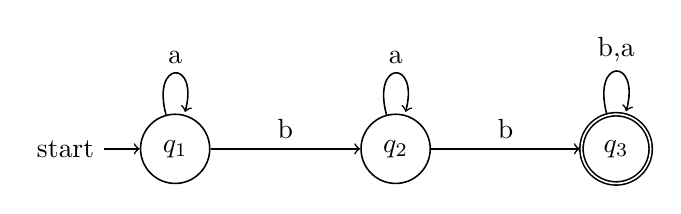
\begin{tikzpicture}[->,auto,node distance=2.8cm,line width=0.2mm]
  \node[initial,state] 			(A)		                 	{$q_1$};
  \node[state]         				(B) [right of=A] 	{$q_2$};
  \node[state,accepting]			(C) [right of=B] 	{$q_3$};

  \path 	(A) edge [loop above] node 	{a} 	(A)
			edge node 			{b}	(B)
	        	(B) edge [loop above] node 	{a} 	(B)
			edge node 			{b} 	(C)
		(C) edge [loop above] node 	{b,a} (C);
\end{tikzpicture}
\caption{Gjenkjenner om et ord har minst to b-er.}
\end{figure}

Hva nå om vi vil slå sammen disse to, og ha en automat som gjenkjenner minst tre a-er og minst to b-er?

\begin{figure}[h!]
\centering
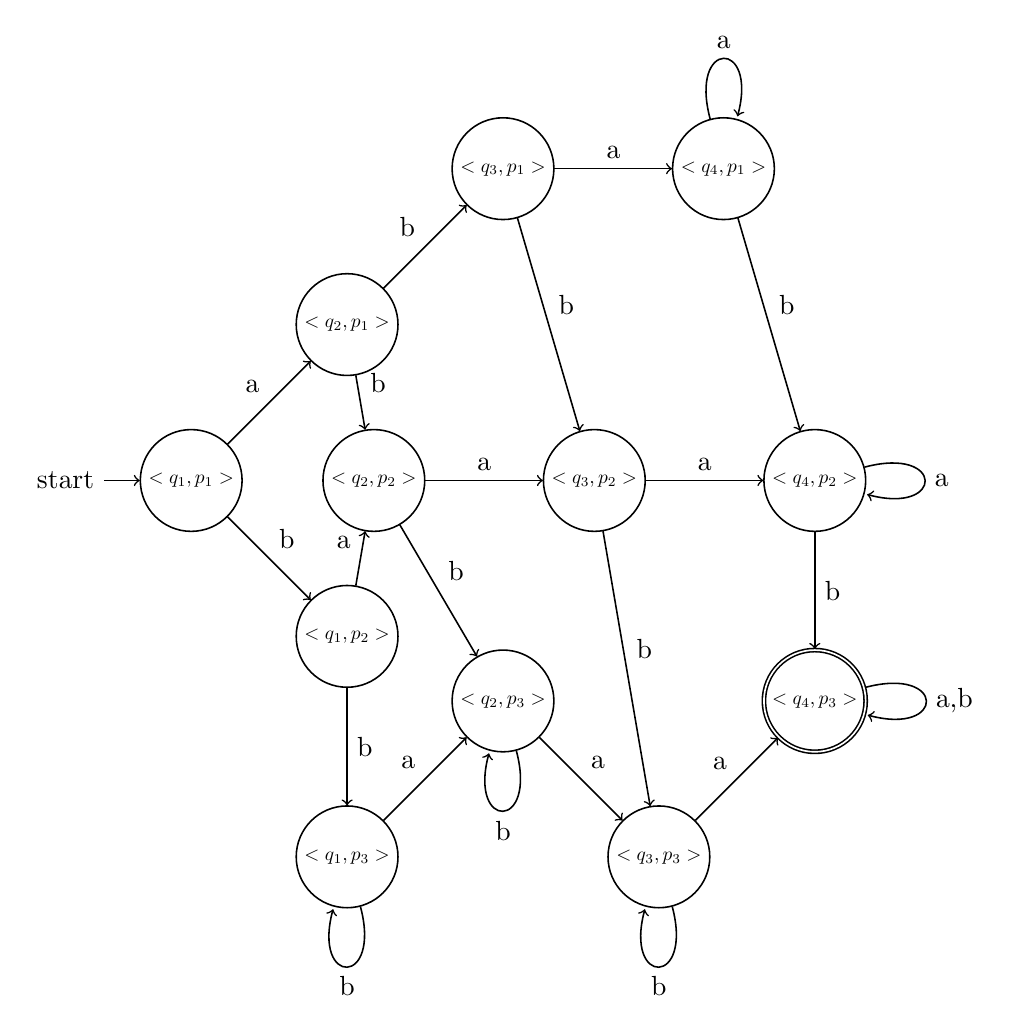
\begin{tikzpicture}[->,auto,node distance=4cm,line width=0.2mm,every state/.style={scale=0.7}]
	\node[initial,state] 				(A)		                 		{$<q_1, p_1>$};
	\node[state]         				(B) [above right of=A] 	{$<q_2, p_1>$};
	\node[state]					(C) [below right of=A] 	{$<q_1, p_2>$};
	\node[state]					(D) [below of=C]		{$<q_1, p_3>$};
	\node[state]					(E) [above right of=D]	{$<q_2, p_3>$};
	\node[state]					(F) [below right of=E]	{$<q_3, p_3>$};
	\node[state,accepting]			(G) [above right of=F]	{$<q_4, p_3>$};
	\node[state]					(H) [above of=G]		{$<q_4, p_2>$};
	\node[state]					(I) [left of=H]			{$<q_3, p_2>$};
	\node[state]					(J) [left of=I]			{$<q_2, p_2>$};
	\node[state]					(K) [above right of=B]	{$<q_3, p_1>$};
	\node[state]					(L) [right of=K]		{$<q_4, p_1>$};

  	\path 	(A) edge node 				{a} 	(B)
				edge node 				{b} 	(C)
			(B) edge node 				{b} 	(K)
				edge node 				{b} 	(J)
			(C) edge node 				{a} 	(J)
				edge node 				{b} 	(D)
			(D) edge node 				{a} 	(E)
				edge [loop below] node 	{b} 	(D)
			(E) edge node 					{a} 	(F)
				edge [loop below] node 	{b} 	(E)
			(F) edge node 					{a} 	(G)
				edge [loop below] node 	{b} 	(F)
			(G) edge [loop right] node 		{a,b} (G)
			(H) edge node 				{b} 	(G)
				edge [loop right] node 		{a} 	(H)
			(I) edge node 					{a} 	(H)
				edge node 				{b} 	(F)
			(J) edge node 					{a} 	(I)
				edge node 				{b}	(E)
			(K) edge node 				{a} 	(L)
				edge node 				{b} 	(I)
			(L) edge [loop above] node 		{a}	(L)
				edge node 				{b} 	(H);
\end{tikzpicture}
\caption{Gjenkjenner om et ord har minst to b-er og minst tre a-er.}
\end{figure}

\subsection{Nondeterministiske}
Hos en DFA er neste tilstand bestemt av inputen. I en NFA har man flervalg, man kan også gå over $\varepsilon$.

\begin{figure}[h!]
\centering
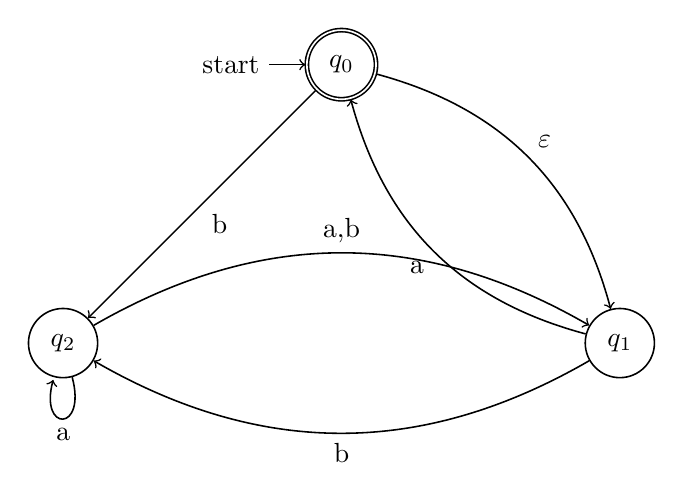
\begin{tikzpicture}[->,auto,node distance=5cm,line width=0.2mm]
  \node[initial,state,accepting] 	(A)                 			{$q_0$};
  \node[state]         				(B) [below right of=A] 	{$q_1$};
  \node[state]					(C) [below left of=A] 	{$q_2$};

  \path 	(A) edge [bend left] node 	{$\varepsilon$} 	(B)
			edge node 			{b} 				(C)
       	 	(B) edge [bend left] node 	{a} 				(A)
			edge [bend left] node 	{b} 				(C)
		(C) edge [loop below] node 	{a} 				(C)
			edge [bend left] node 	{a,b} 			(B);
\end{tikzpicture}
\caption{Eksempel på en NFA.}
\end{figure}

\theoremstyle{mytheoremstyle}
\newtheorem{nfa}{Definisjon}[section]
\begin{nfa}
En \textbf{nondeterministic finite automata} er et 5-tuppel $(Q, \Sigma, \delta, q_0, F)$, hvor:
\begin{enumerate}
	\item{$Q$ er tilstandene.}
	\item{$\Sigma$ er alfabetet.}
	\item{$\delta : Q \times \Sigma_{\epsilon} \longrightarrow P(Q)$}
	\item{$q_0 \in Q$ er starttilstanden.}
	\item{$F \subseteq Q$ er de aksepterte tilstandene.}
\end{enumerate}
\end{nfa}

\subsection{Pumpelemma}
\begin{enumerate}
	\item{Stringen lager en sti mellom tilstandene.}
	\item{Anta at antall tilstander er $p$.}
	\item{Enhver string lengere enn $p$ må gå $n$ loop.}
	\item{Treffer tilstand vi har vært borte i fra før.}
\end{enumerate}

\theoremstyle{mytheoremstyle}
\newtheorem{pumpe}{Definisjon}[section]
\begin{pumpe}
Anta at vi har en DFA $D$ med $d$ tilstander og et ord $w$ av lengde $n$ som blir akseptert av $D$. Om $n > d$, så kan vi dele $w$ opp i $w = xyz$ med lengden av $xy \leq n + 1$, $y$ ikke tom og der samtlige $x(y)*z$ blir akseptert.
\end{pumpe}

\subsection{Pushdown automata - PDA}
En PDA består av tilstander, en start, transisjoner og aksepterende.
Starten er en starttilstand og en tom stakk. Transisjoner er som følger:


\begin{center}
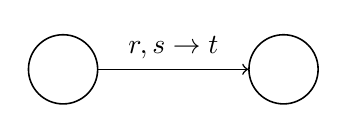
\begin{tikzpicture}[->,auto,node distance=2.8cm,line width=0.2mm]
  \node[state] 				(A)             		    	{};
  \node[state]         			(B) [right of=A] 	{};

  \path 	(A) edge node {$r,s \rightarrow t$} (B);
\end{tikzpicture}
\end{center}

Hvor $r,s$ er forutsetninger og $t$ er aksjonen. Deler dette opp i to:
\begin{enumerate}
	\item{Vokter: symbol lest, symbol øverst på stakken/tas av på stakken.}
	\item{Aksjon: nytt symbol på stakken.}
\end{enumerate}

Bruker også $\varepsilon$. Akseptering skjer med aksepterende tilstand eller en tom stakk.

\subsubsection{Chomskys normalform}
\begin{itemize}
	\item{Enhver CFG kan skrives ved bruk av regler: $A \longrightarrow BC$, $D \longrightarrow d$}
	\item{Forgrening for variable.}
	\item{Unært (rett fram) for terminaler.}
\end{itemize}

\section{Regulære Uttrykk}
Ta $\Sigma = \{a,b\}$. De regulære uttrykkene gir delmengder av stringer i $\{a, b\}$.
\begin{itemize}
	\item{$\emptyset$ -- tom delmengde.}
	\item{$\epsilon$ -- $\{\epsilon\}$}
	\item{a -- \{a\}}
	\item{b -- \{b\}}
	\item{union}
	\item{konkatinering}
	\item{kleene stjerne}
\end{itemize}

Et regulært språk er en delmengde av stringen som en DFA kan akseptere. Regulære uttrykk = regulære språk.

\subsection{DFA til regulært uttrykk}

\begin{figure}[h!]
\centering
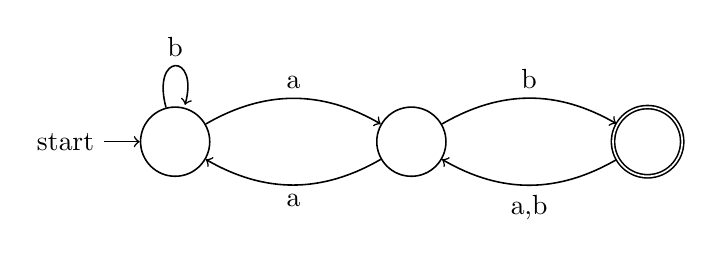
\begin{tikzpicture}[->,auto,node distance=3cm,line width=0.2mm]
  \node[initial,state] 			(A)             		    		{};
  \node[state]         				(B) [right of=A] 		{};
  \node[state,accepting]			(C) [right of=B]	 	{};

  \path 	(A) edge [bend left] node 	{a} (B)
			edge [loop above] node {b} (C)
       	 	(B) edge [bend left] node	{a} (A)
			edge [bend left] node 	{b} (C)
		(C)	edge [bend left] node 	{a,b} (B);
\end{tikzpicture}
\end{figure}

Trenger fire steg:

\paragraph{Steg 1} legger til starttilstand og aksepterende over $\varepsilon$.
\begin{figure}[h!]
\centering
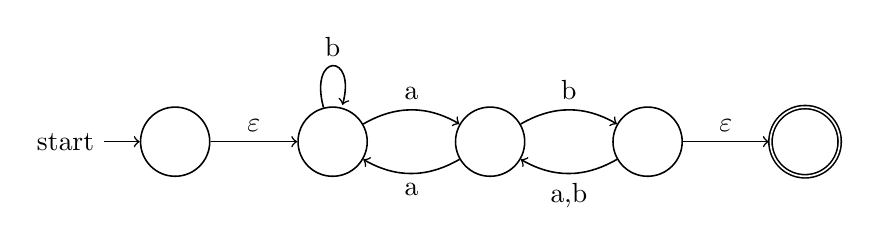
\begin{tikzpicture}[->,auto,node distance=2cm,line width=0.2mm]
  \node[state,initial] 			(A)                 			{};
  \node[state]         				(B) [right of=A] 		{};
  \node[state]					(C) [right of=B]	 	{};
  \node[state]					(D) [right of=C]	 	{};
  \node[state,accepting]			(E) [right of=D]	 	{};

  \path 	(A) edge node 			{$\varepsilon$} 	(B)
		(B)	edge [loop above] node {b} 				(B)
        		(B) edge [bend left] node 	{a} 				(C)
		(C)	edge [bend left] node 	{a} 				(B)
		(C)	edge [bend left] node 	{b} 				(D)
		(D)	edge [bend left] node 	{a,b} 			(C)
			edge node 			{$\varepsilon$} 	(E);
\end{tikzpicture}
\end{figure}

\paragraph{Steg 2} bruker GNFA (reg.exp på pilene) og tar vekk en tilstand, så reparer.
\begin{figure}[h!]
\centering
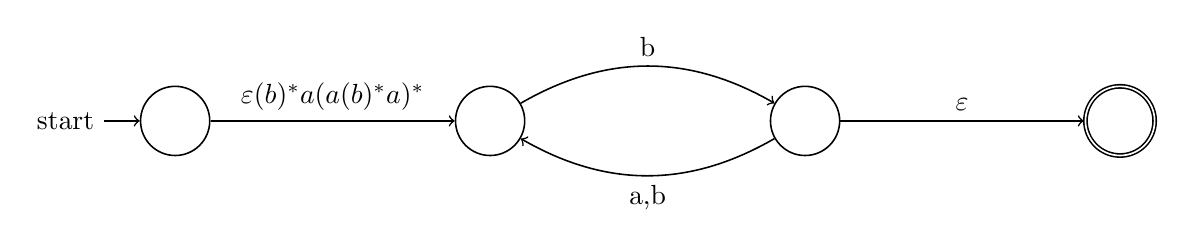
\begin{tikzpicture}[->,auto,node distance=4cm,line width=0.2mm]
  \node[state,initial] 			(A)                 			{};
  \node[state]         				(B) [right of=A] 		{};
  \node[state]					(C) [right of=B]	 	{};
  \node[state,accepting]			(D) [right of=C]	 	{};

  \path 	(A) 	edge node {$\varepsilon (b)^*a(a(b)^*a)^*$} (B)
		(B)	edge [bend left] node {b} (C)
		(C)	edge [bend left] node {a,b} (B)
		(C)	edge node {$\varepsilon$} (D);
\end{tikzpicture}
\end{figure}

\paragraph{Steg 3} tar vekk en ny tilstand.
\begin{figure}[h!]
\centering
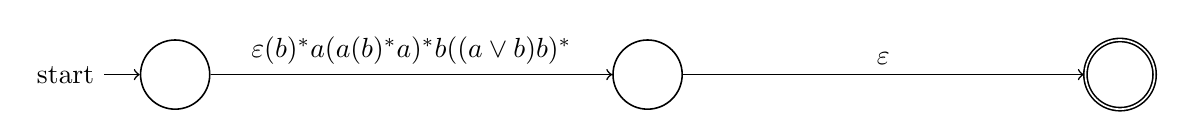
\begin{tikzpicture}[->,auto,node distance=6cm,line width=0.2mm]
  \node[state,initial] 			(A)          		       		{};
  \node[state]         				(B) [right of=A] 		{};
  \node[state,accepting]			(C) [right of=B]	 	{};

  \path 	(A) edge node {$\varepsilon (b)^*a(a(b)^*a)^*b((a \vee b)b)^*$} (B)
		(B) edge node {$\varepsilon$} (C);
\end{tikzpicture}
\end{figure}

\paragraph{Steg 4} tar bort den siste tilstanden.
\begin{figure}[h!]
\centering
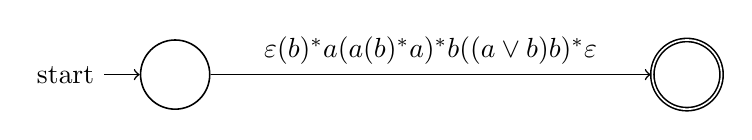
\begin{tikzpicture}[->,auto,node distance=6.5cm,line width=0.2mm]
  \node[state,initial] 			(A)                 		{};
  \node[state,accepting]        		(B) [right of=A] 	{};

  \path 	(A) edge node {$\varepsilon (b)^*a(a(b)^*a)^*b((a \vee b)b)^*\varepsilon$} (B);
\end{tikzpicture}
\end{figure}

Vi får da det hele regulære uttrykket: $$\epsilon(b)^*a(a(b)^*a)^*b((a \vee b)b)^*\epsilon$$


\subsection{Fra NFA til reg.ex.}
\begin{figure}[h!]
\centering
\begin{tikzpicture}[->,auto,node distance=5cm,line width=0.2mm]
  \node[state] 		(A)                 			{};
  \node[state]      	(B) [right of=A] 		{};
  \node[state]		(C) [above right of=A] 	{};

  \path 	(A) edge node {T} (B)
			edge node {S} (C)
        		(B) edge node {V} (C)
		(C) edge [loop above] node {U} (C);
\end{tikzpicture}
\caption{En NFA.}
\label{nfareg}
\end{figure}

\begin{figure}[h!]
\centering
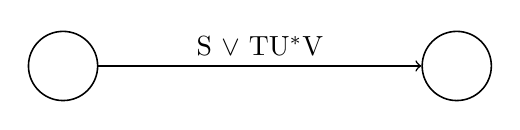
\begin{tikzpicture}[->,auto,node distance=5cm,line width=0.2mm]
  \node[state] 		(A)                 			{};
  \node[state]      	(B) [right of=A] 		{};

  \path 	(A) edge node {S $\vee$ TU$^*$V} (B);
\end{tikzpicture}
\caption{Figur \ref{nfareg} som regex.}
\label{regex}
\end{figure}

\section{Kontekstfrie språk}
\begin{enumerate}
	\item{Gramatikk -- CFG -- kontekstfire språk.}
	\item{Automat med stakk -- PDA -- pushdown automata.}
\end{enumerate}

\paragraph{Eksempel på CFG}
Språk: $(((())))$

\begin{itemize}
	\item{Variable: $S$ og $A$.}
	\item{Terminaler: $($ og $)$.}
	\item{Startsymbol: $S$.}
	\item{Regler (omskrivningsregler): $S \rightarrow A$, $A \rightarrow AA$, $A \rightarrow (A)$, $A \rightarrow ()$}
	\item{Utledning: 
\begin{spacing}{0.4}$$ S $$
$$\line(1,0){30}$$
$$ A $$
$$\line(1,0){35}$$
$$ AA $$
$$\line(1,0){40}$$
$$() A$$
$$\line(1,0){45}$$
$$() (A)$$
$$\line(1,0){50}$$
$$() (())$$\end{spacing}}
Lager uttrykk som ()(()).
\end{itemize}

Regler: $v.s. \rightarrow h.s.$
Venstresiden inneholder nøyaktig ett symbol. Dette er begrunnelsen for at språk er kontekstfri. Symbolet er en variabel.
Høyresiden er en string av symboler. Utledningen fortsetter omskrivningene til vi bare har terminale symboler.

\begin{figure}[h!]
\centering
\begin{tikzpicture}[every node/.style={},level 2/.style={sibling distance=20mm},level 3/.style={sibling distance=10mm}, level distance=30pt]
\node {S}
	child { node{A} 
		child { node {A} 
			child { node {(} }
			child { node {)} }
		}
		child { node {A} 
			child { node {(} }
			child { node {A} 
				child { node {(} }
				child { node {)} }
			}
			child { node {)} }
		}
	};
\end{tikzpicture}
\caption{Utledningen i treform.}
\end{figure}

Begynner med $S$. Variablene er interne noder, og terminalene er løvnoder.

\section{Turing maskiner}
\subsection{Turing analyse}

Beregninger på rutepapir. Trenger ekstra blanke ruter. Tillater flere tilstander. Klarer seg med én aktiv rute. Beregning gjøres på tape. Bevege aktiv rute høyre/ventre/stopp. Klarer seg med to symboler i alfabetet. Kan utføre hvilken som helst beregning slik.

\subsection{Turing maskinen}
Forskjellen mellom en finite automata og en turing maskin er:
\begin{itemize}
	\item{En turing maskin kan både lese og skrive til og fra en tape.}
	\item{Lese-/skrivehodet kan bevege seg til både høyre og venstre.}
	\item{Tapen er uendelig.}
	\item{Aksepterende og avvisende tilstand trår i kraft umiddelbart.}
\end{itemize}

\begin{center}
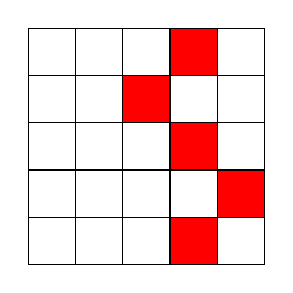
\begin{tikzpicture}[x=0.6cm,y=0.6cm]

\foreach \i in {0 , 1 , 2, 3, 4}
{\foreach \j in {0 , 1 , 2, 3, 4}
{\draw (\i,\j) rectangle +(1,1);}}

\draw[fill=red] (3,4) rectangle +(1,1) ;
\draw[fill=red] (2,3) rectangle +(1,1) ;
\draw[fill=red] (3,2) rectangle +(1,1) ;
\draw[fill=red] (4,1) rectangle +(1,1) ;
\draw[fill=red] (3,0) rectangle +(1,1) ;

\end{tikzpicture}
\end{center}

Tapen er den horisontale raden og aktiv rute er markert med rød. Tid er x-aksen og rom er y-aksen.


\begin{figure}[h!]
\centering
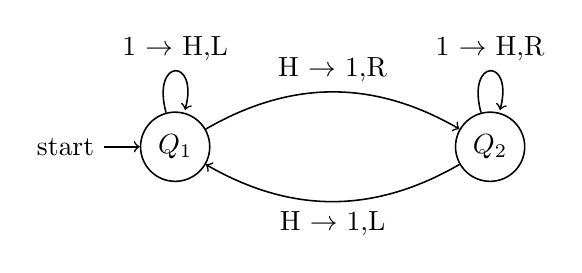
\begin{tikzpicture}[->,auto,node distance=4cm,line width=0.2mm]
  \node[initial,state] 		(A)                   	 	{$Q_1$};
  \node[state]         			(B) [right of=A] 	{$Q_2$};

  \path 	(A) edge [bend left] node {H $\rightarrow$ 1,R} (B)
		(A) edge [loop above] node {1 $\rightarrow$ H,L} (A)
        		(B) edge [bend left] node {H $\rightarrow$ 1,L} (A)
		(B) edge [loop above] node {1 $\rightarrow$ H,R} (B);
\end{tikzpicture}
\caption{Eksempel på en Turing maskin.}
\end{figure}

I eksempel 10 ser vi en TM med to tilstander: $Q_1$ og $Q_2$. Denne tar enten inn $1$ eller $H$ (blank). Den kan lese $1$, da skriver den $H$ og går til venstre (left, L), da havner den i samme tilstand $Q_1$. Så kan den lese $H$, skrive $1$ og gå til høyre (right, R), og havner i tilstand $Q_2$.

\theoremstyle{mytheoremstyle}
\newtheorem{tm}{Definisjon}[section]
\begin{tm}
En \textbf{TM} er et 7-tuppel $(Q, \Sigma, \Gamma, \delta, q_0, q_{accept}, q_{reject})$
\begin{enumerate}
	\item{$Q$ er tilstandene,}
	\item{$\Sigma$ er input alfabetet som ikke holder blanke,}
	\item{$\Gamma$ er alfabetet på tapen -- inkludert blanke,}
	\item{$\delta : Q \times \Gamma \rightarrow Q \times \Gamma \times \{L, R\}$ er funksjonen for transisjonene,}
	\item{$q_0 \in Q$ er starttilstanden,}
	\item{$q_{accept} \in Q$ er aksepterende tilstand, og}
	\item{$q_{reject} \in Q$ er avvist tilstand. Hvor $q_{reject} \neq q_{accept}$}.
\end{enumerate}
\end{tm}

\subsubsection{Konfigurasjon}
Når en Turing maskin beregner vil endringer skje i gjeldene tilstand, gjeldene innhold på tapen og gjeldende posisjon på lokasjonen til hodet. Disse tre gjenstandene kalles en \textbf{konfigurasjon} av Turing maskinen.

Konfigurasjonen er skrevet som: $uqv$, hvor $q$ er tilstanden, $u$ og $v$ er to stringer i $\Gamma$. $q$ er gjeldende tilstand og $uv$ er gjeldende innhold på tapen. Gjeldende posisjon for hodet er $v$.

Spesielle hendelser kan oppstå når hodet er på en av endelsene i konfigurasjonen. For en hendelse til venstre: $q_ibv$ gir $q_jcv$ hvis transisjonen beveger seg til venstre. Og den gir $cq_jv$ for en transisjon som går til høyre. For den som slutter til høyre i konfigurasjonen $uaq_i$ er ekvivalent med $uaq_i\textvisiblespace$, fordi vi antar at resten av tapen er blank.

Startkonfigurasjonen for $\mathcal{M}$ på input $w$ er konfigurasjonen $q_0w$, dette indikerer at maskinen er i starttilstanden $q_0$ med hodet lengst til venstre på tapen. I en aksepterende konfigurasjon, er tilstanden $q_{accept}$. Og for en avvisende konfigurasjon er den $q_{reject}$. Aksepterende og avvisende konfigurasjoner er stagnerende konfigurasjoner (halting) og gir ingen flere konfigurasjoner.

En TM $\mathcal{M}$ aksepterer input $w$ hvis en sekvens av konfigurasjoner $C_1, C_2, \dots,C_k$ eksisterer, hvor:
\begin{enumerate}
	\item{$C_1$ er startkonfigurasjonen på input $w$,}
	\item{hver $C_i$ gir $C_{i+1}$, og}
	\item{$C_k$ er en aksepterende konfigurasjon.}
\end{enumerate}

\subsubsection{Grunnleggende Turing maskiner}

\paragraph{Skrive ord}
\begin{description}
\item[Alfabet]: a, b, 0 -- 0 er blank.
\item[Spesifikasjon]: skriver $abba$ og stopper.
\end{description}
\begin{figure}[h!]
\centering
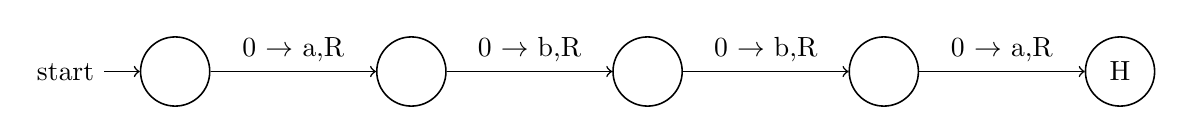
\begin{tikzpicture}[->,auto,node distance=3cm,line width=0.2mm]
  \node[initial,state] 	(A)	                    	{};
  \node[state]         		(B) [right of=A] 	{};
  \node[state]         		(C) [right of=B] 	{};
  \node[state]         		(D) [right of=C] 	{};
  \node[state]         		(E) [right of=D] 	{H};

  \path 	(A) edge node {0 $\rightarrow$ a,R} (B)
		(B) edge node {0 $\rightarrow$ b,R} (C)
       	 	(C) edge node {0 $\rightarrow$ b,R} (D)
		(D) edge node {0 $\rightarrow$ a,R} (E);
\end{tikzpicture}
\end{figure}

\paragraph{Bytte bokstaver}
\begin{description}
\item[Alfabet]: a, b, 0 -- 0 er blank.
\item[Spesifikasjon]: bytter b mot a og motsatt til den treffer en blank.
\end{description}
\begin{figure}[h!]
\centering
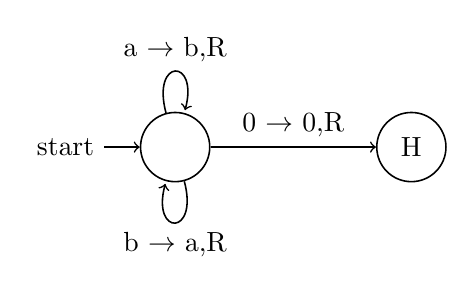
\begin{tikzpicture}[->,auto,node distance=3cm,line width=0.2mm]
  \node[initial,state] 		(A)                    		{};
  \node[state]         			(B) [right of=A] 	{H};

  \path 	(A) edge [loop above] node {a $\rightarrow$ b,R} (A)
		(A) edge [loop below] node {b $\rightarrow$ a,R} (A)
        	(A) edge node {0 $\rightarrow$ 0,R} (B);
\end{tikzpicture}
\end{figure}

\subsection{Flittige bevere}
Maskiner i alfabetet $0,1$ -- 0 er blank. En bever stopper. 

N-bever: bever med N tilstander + stopptilstand.
\begin{itemize}
\item{For Turing maskiner i 0,1 med N tilstander + stopp:}
\begin{itemize}
\item{$2N$ voktere.}
\item{Hver transisjon kan utføre $2(N+1)2$ handlinger.}
\item{Det er $(4N + 4)^{2N}$ slike maskiner.}
\item{Noen av disse stopper, andre stopper ikke.}
\end{itemize}
\item{Flittig N-bever: N-bever som produserer flest antall 1ere.}
\end{itemize}

Bever funksjonen: $\beta(1) = 1, \beta(2) = 4, \beta(3) = 6, \beta(4) = 13, \beta(5) \geq 4098$

\begin{figure}[h!]
\centering
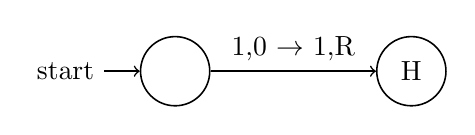
\begin{tikzpicture}[->,auto,node distance=3cm,line width=0.2mm]
  \node[initial,state] 		(A)               	     	{};
  \node[state]         			(B) [right of=A] 	{H};

  \path 	(A) edge node {1,0 $\rightarrow$ 1,R} (B);
\end{tikzpicture}
\caption{Flittig 1-bever -- $\beta(1) = 1$}
\end{figure}

\begin{figure}[h!]
\centering
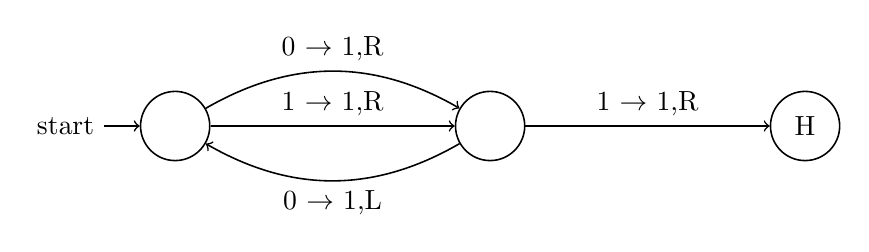
\begin{tikzpicture}[->,auto,node distance=4cm,line width=0.2mm]
  \node[initial,state] 		(A)                 	   	{};
  \node[state] 				(B) [right of=A]    	{};
  \node[state]         			(C) [right of=B] 	{H};

  \path 	(A) edge node {1 $\rightarrow$ 1,R} (B)
		(A) edge [bend left] node {0 $\rightarrow$ 1,R} (B)
		(B) edge [bend left] node {0 $\rightarrow$ 1,L} (A)
		(B) edge node {1 $\rightarrow$ 1,R} (C);
\end{tikzpicture}
\caption{Flittig 2-bever -- $\beta(2) = 4$}
\end{figure}

\begin{figure}[h!]
\centering
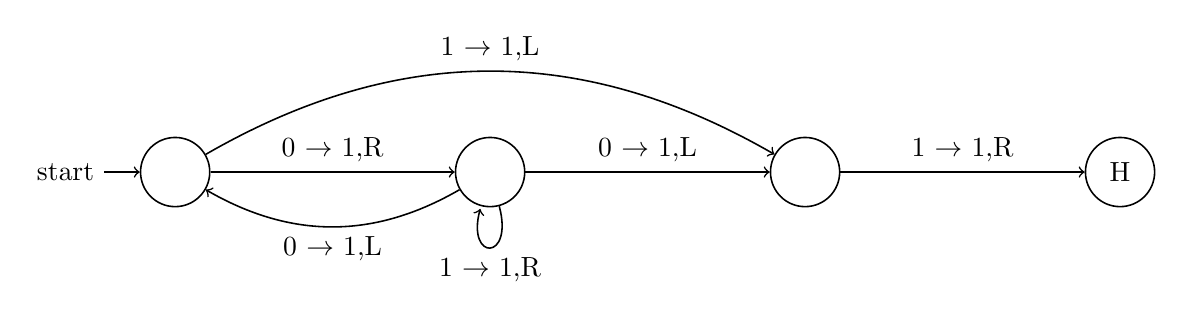
\begin{tikzpicture}[->,auto,node distance=4cm,line width=0.2mm]
  \node[initial,state] 		(A)                 	   	{};
  \node[state] 				(B) [right of=A]    	{};
  \node[state] 				(C) [right of=B]    	{};
  \node[state]         			(D) [right of=C] 	{H};

  \path 	(A) edge node {0 $\rightarrow$ 1,R} (B)
		(A) edge [bend left] node {1 $\rightarrow$ 1,L} (C)
		(B) edge [bend left] node {0 $\rightarrow$ 1,L} (A)
		(B) edge [loop below] node {1 $\rightarrow$ 1,R} (B)
		(B) edge node {0 $\rightarrow$ 1,L} (C)
		(C) edge node {1 $\rightarrow$ 1,R} (D);
\end{tikzpicture}
\caption{Flittig 3-bever -- $\beta(3) = 6$}
\end{figure}

\begin{figure}[h!]
\centering
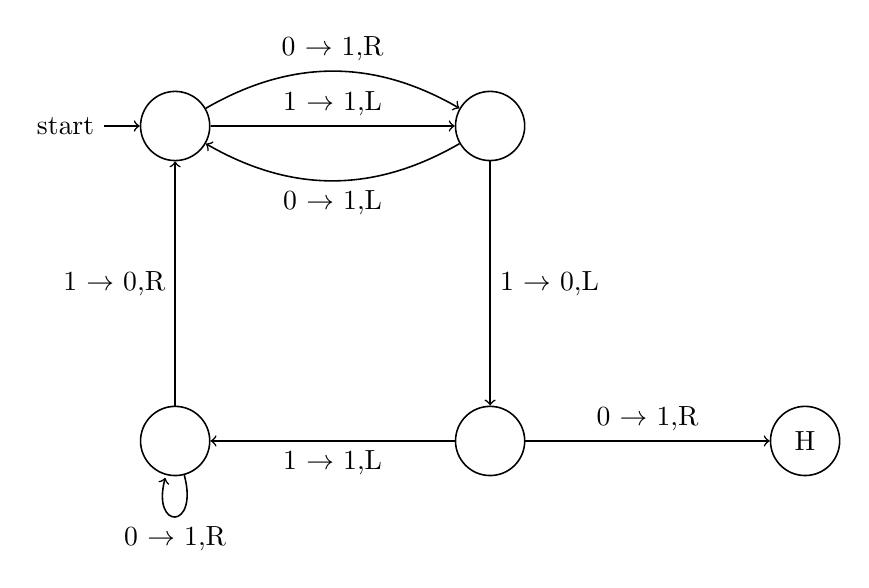
\begin{tikzpicture}[->,auto,node distance=4cm,line width=0.2mm]
  \node[initial,state] 		(A)            		        	{};
  \node[state] 				(B) [below of=A]   	{};
  \node[state] 				(C) [right of=A]    	{};
  \node[state] 				(D) [below of=C] 	{};
  \node[state]         			(E) [right of=D] 	{H};

  \path 	(A) edge node {1 $\rightarrow$ 1,L} (C)
		(A) edge [bend left] node {0 $\rightarrow$ 1,R} (C)
		(C) edge [bend left] node {0 $\rightarrow$ 1,L} (A)
		(B) edge node {1 $\rightarrow$ 0,R} (A)
		(B) edge [loop below] node {0 $\rightarrow$ 1,R} (B)
		(D) edge node {1 $\rightarrow$ 1,L} (B)
		(C) edge node {1 $\rightarrow$ 0,L} (D)
		(D) edge node {0 $\rightarrow$ 1,R} (E);
\end{tikzpicture}
\caption{Flittig 4-bever -- $\beta(4) = 13$}
\end{figure}

\paragraph{Beverfunksjonen er ikke beregnbar}
La $f(n)$ være en beregnbar funksjon.
\begin{itemize}
\item{TM med $k$ tilstander i alfabetet $0$, $1$.}
\item{Starter beregningen til venstre for $n$ 1ere -- ellers bare 0.}
\item{Stopper beregningen til venstre for $f(n)$ 1ere -- ellers bare 0.}
\item{Antar at $f(n) > n^2$ -- $f$ vokser raskere enn lineært.}
\item{Antar $f$ er strengt voksende -- $f(n+1) > f(n)$.}
\end{itemize}

$f(f(n))$ kan beregnes med $2k$ tilstander. Tallet $f(f(n))$ kan beregnes med $n+2k$ tilstander fra blank. $\beta(n+2k) \geq f(f(n)) \geq f(n^2) \succ f(n+2k)$

\subsection{Nondeterministisk Turing maskin}
På hvilket som helst punkt i beregningen kan maskinen fortsette i forskjellige retninger. Transisjonsfunksjon for en NTM:
$$\delta : Q \times \Gamma \rightarrow \mathcal{P}(Q \times \Gamma \times \{L,R\}).$$

Beregningen av en NTM er et tre med grener som tilsvarer de forskjellige mulighetene for maskinen.

\paragraph{Teorem} Hver NTM har en ekvivalent deterministisk TM.

Simulerer en NTM $\mathcal{N}$ med en deterministisk TM $\mathcal{D}$. Tanken bak simuleringen er at $\mathcal{D}$ må prøve alle mulige grener av $\mathcal{N}$. Hvis $\mathcal{D}$ noen gang finner en aksepterende tilstand i en av grenene, aksepter. Ellers vil $\mathcal{D}$ sin simulering ikke terminere.

\paragraph{Bevis} Simulerende $\mathcal{D}$ har tre taper. Dette er ekvivalent med å ha en tape. Tape 1 har alltid input string og stopper aldri. Tape 2 er en kopi av $\mathcal{N}$ sin tape av en gren i dens nondeterministiske beregning. Tape 3 holder styr på lokasjonen til $\mathcal{D}$ i $\mathcal{N}$ sitt tre.

Først vurderer vi data-representasjonen på tape 3. Hver node i treet kan ha max. $b$ barn, hvor $b$ er størrelsen av det største settet som mulig av valg gitt av $\mathcal{N}$ sin transisjonsfunksjon. For hver node i treet gir vi en adresse som er en string fra alfabetet $\Gamma_b = \{1,2,\dots,b\}$. Gir adressen 231 til noden vi finner ved å starte ved roten, går så til 2. barn, så til den nodens 3. barn, og til slutt dens 1. barn. Tape 3 inneholder en string over $\Gamma_b$. Den tomme stringen adresserer roten i treet.
\newline
\newline
Beskrivelse av $\mathcal{D}$:
\begin{enumerate}
\item{Tape 1 inneholder input $w$, tape 2 og tape 3 er tomme.}
\item{Kopierer tape 1 til tape 2 og initialiserer stringen på tape 3 til $\varepsilon$.}
\item{Bruker tape 2 til å simulere $\mathcal{N}$ med input $w$ på en gren av den nondeterministiske beregningen. Før hvert steg av $\mathcal{N}$, konstanter neste symbol på tape 3 for å bestemme hvilket valg blant de som $\mathcal{N}$ tillater i sin transisjonsfunksjon. Hvis det er ingen symboler igjen på tape 3 eller om det nondeterministiske valget ikke er gyldig, aborter grenen og gå til steg 4. Gå også til steg 4 hvis en avvisende konfigurasjon inntreffer. Hvis en aksepterende konfigurasjon inntreffer, aksepter.}
\item{Erstatt stringen på tape 3 med neste. Simuler neste gren ved å gå til steg 2.}
\end{enumerate}

\section{Avgjørbar}
Vi starter med beregningsproblemer knyttet til finite automata. Bruker algoritmer for å teste om automaten aksepterer en string, om språket er tomt og om to automater er ekvivalente.

\subsection{For DFA}
\paragraph{Eksempel} Aksepteringsproblemet for DFA er ved testing om en spesifik string kan bli uttrykt som språket $A_{DFA}$.
Dette språket inneholder enkoding for alle DFAer tilsammen med stringer som blir akseptert av DFAene. La
\begin{center}
$A_{DFA} = \{\langle \mathcal{B},w \rangle | \mathcal{B} $ er en DFA som aksepterer input string $w$\}.
\end{center}

Problemet med å teste om en DFA $\mathcal{B}$ aksepterer input $w$ er det samme som å teste om $\langle \mathcal{B},w \rangle$ er et medlem av språket $A_{DFA}$. En TM $\mathcal{M}$ bestemmer $A_{DFA}$

$\mathcal{M}$ = på input $\langle \mathcal{B},w \rangle$, hvor $\mathcal{B}$ er en DFA og $w$ er en string:
\begin{enumerate}
\item{Simuler $\mathcal{B}$ på input $w$.}
\item{Hvis simuleringen ender i aksepterende tilstand, aksepter. Ellers, avvis.}
\end{enumerate}

\paragraph{Bevis} Undersøke $\langle \mathcal{B},w \rangle$. Det er en representasjon av en DFA $\mathcal{B}$ sammen med en string $w$. Når $\mathcal{M}$ får dens input, $\mathcal{B}$ velger om den representerer en DFA $\mathcal{B}$ og en tring $w$. Hvis ikke avviser $\mathcal{M}$. $\mathcal{M}$ følger simuleringen direkte. Holder styr på $\mathcal{B}$ sin gjeldende tilstand og $\mathcal{B}$ sin gjeldende posisjon i input $w$ ved å skrive informasjon på tapen.

\subsection{For NFA}
Vi kan også bevise det samme for en NFA. La
\begin{center}
$A_{NFA} = \{\langle \mathcal{B},w \rangle | \mathcal{B}$ er en NFA som aksepterer på input string $w$\}.
\end{center}

\paragraph{Teorem} $A_{NFA}$ er et bestembart språk.
\paragraph{Bevis} En TM $\mathcal{N}$ bestemmer $A_{NFA}$. La $\mathcal{N}$ bruke $\mathcal{M}$ som en sub-rutine. Fordi $\mathcal{M}$ er designet for å jobbe med DFAer, $\mathcal{N}$ konverterer først NFAen til en DFA, før den gir den til $\mathcal{M}$.

$\mathcal{N}$ = på input $\langle \mathcal{B},w \rangle$, hvor $\mathcal{B}$ er en NFA og $w$ er en string:
\begin{enumerate}
\item{Koverter NFA $\mathcal{B}$ til en ekvivalent DFA $\mathcal{C}$, ved å bruke prosedyre for konvertering.}
\item{Kjør TM $\mathcal{M}$ på input $\langle \mathcal{C},w \rangle$}.
\item{Hvis $\mathcal{M}$ aksepterer, aksepter. Ellers, avvis.}
\end{enumerate}

Ved å kjøre TM $\mathcal{M}$ i steg 2 betyr å i steg 2 betyr å inkorporere $\mathcal{M}$ til designet $\mathcal{N}$ som en sub-prosedyre.

\subsection{For Regulært Uttrykk}
Likedan kan vi se om et reg.ex. genererer en gitt string. La
\begin{center}
$A_{REX} = \{\langle \mathcal{R},w \rangle | \mathcal{R}$ er et reg.ex. som genererer string $w$ \}.
\end{center}

\paragraph{Bevis} TM $\mathcal{P}$ bestemmer $A_{REX}$.

$\mathcal{P}$ = på input $\langle \mathcal{R},w \rangle$, hvor $\mathcal{R}$ er et reg.ex. og $w$ en string:
\begin{enumerate}
\item{Konverter reg.ex. $\mathcal{R}$ til en ekvivalent NFA $\mathcal{A}$.}
\item{Kjør TM $\mathcal{N}$ på input $\langle \mathcal{A},w \rangle$.}
\item{Hvis $\mathcal{N}$ aksepterer, aksepter. Ellers, avvis.}
\end{enumerate}

\section{Redusering}
En reduksjon er en måte å konvertere et problem til et annet, slik at løsningen på det andre problemet kan brukes til å løse det første.

\subsection{Stoppeproblemet}
Ta for eksempel stoppeproblemet. Bruker da ikke-avgjørbarheten til $A_{TM}$ for å vise ikke-avgjørbarheten til $HALT_{TM}$. La
\begin{center}
$HALT_{TM} = \{\langle \mathcal{M}, w \rangle | \mathcal{M}$ er en TM og $\mathcal{M}$ stagnerer på input $w$ \}.
\end{center}

\paragraph{Teorem} $HALT_{TM}$ er ikke-avgjørbart.
\paragraph{Idé} Anta at man har en TM $\mathcal{R}$ som avgjør $HALT_{TM}$. Med $\mathcal{R}$ kan man teste om $\mathcal{M}$ stopper på $w$ eller ikke. Hvis $\mathcal{R}$ indikerer at $\mathcal{M}$ ikke stopper på $w$ -- avvis, fordi $\langle \mathcal{M}, w \rangle$ er ikke i $A_{TM}$. Hvis $\mathcal{R}$ indikerer at $\mathcal{M}$ stopper på $w$, kan man simulere uten fare for loop. Hvis TM $\mathcal{R}$ eksisterer kan vi avgjøre $A_{TM}$, men vi vet at $A_{TM}$ er ikke-avgjørbart. Ved denne motsigelsen kan vi konkludere med at $\mathcal{R}$ ikke eksisterer -- derfor er $HALT_{TM}$ ikke-avgjørbart.

\paragraph{Bevis} For motsigelsens skyld anta at TM $\mathcal{R}$ avgjør $HALT_{TM}$. Konstruerer TM $\mathcal{S}$ for å avgjøre $A_{TM}$.

$\mathcal{S}$ = på input $\langle \mathcal{M}, w \rangle$, en enkoding av TM $\mathcal{M}$ og en string $w$:
\begin{enumerate}
\item{Kjør TM $\mathcal{R}$ på input $\langle \mathcal{M}, w \rangle$}.
\item{Hvis $\mathcal{R}$ avviser, avvis.}
\item{Hvis $\mathcal{R}$ aksepterer, simuler $\mathcal{M}$ på $w$ til den stopper.}
\item{Hvis $\mathcal{M}$ aksepterer, aksepter. Hvis $\mathcal{M}$ avviser, avvis.}
\end{enumerate}

Hvis $\mathcal{R}$ avgjør $HALT_{TM}$, så vil $\mathcal{S}$ avgjøre $A_{TM}$. Siden vi vet at $A_{TM}$ er ikke-avgjørbar, så må $HALT_{TM}$ også være ikke-avgjørbar.


\section{Kompleksitet i tid}
\paragraph{Eksempel} Gitt språket $A = \{0^k1^k | k \geq 0\}$.
$A$ er et avgjørbart språk. Hvor mye tid bruker en single-tape TM på å avgjøre $A$? La TM hete $M_1$.

$M_1$ = på intput string $w$:
\begin{enumerate}
\item{Søker på tapen og avviser om 0 blir funnet til høyre for 1.}
\item{Gjentar om både 0 og 1 er igjen på tapen.}
\item{Søker gjennom tapen og krysser bort enkel 0 og enkel 1.}
\item{Hvis det er flere 0er igjen etter alle 1ere er krysset av, eller motsatt, avvis. Hvis hele inputen er krysset av, aksepter.}
\end{enumerate}

I en \textbf{worst-case analyse}, antar vi lengst kjøretid for alle inputs av en gitt lengde. I en \textbf{gjennomsnittsanalyse} ser vi på snittet av kjøretiden for inputs med en gitt lengde. 

\theoremstyle{mytheoremstyle}
\newtheorem{tid}{Definisjon}[section]
\begin{tid}
La $M$ være en deterministisk TM som stopper for alle inputs. \textbf{Kjøretiden} for $M$ er funksjonen
$$f:\mathcal{N \rightarrow N}$$
hvor $f(n)$ er max. lengde på steg $M$ bruker for hvilken som helst input av lengde $n$. Hvis $f(n)$ er kjøretiden til $M$, er $M$ en $f(n)$-tid TM.
\end{tid}

\subsection{P-klassen}
\theoremstyle{mytheoremstyle}
\newtheorem{ptid}{Definisjon}[section]
\begin{ptid}
P er klassen av språk som er avgjort ved \textbf{polynom-tid} for en deterministisk single-tape TM.
$$P = \bigcup_{k} TIME (n^k)$$

\begin{enumerate}
\item{P er en invariant for alle modeller for beregning som er polynom ekvivalent til den deterministiske single-tape Turing maskinen, og}
\item{P svarer til gruppen av problemer som realistisk sett kan løses på en datamaskin.}
\end{enumerate}
\end{ptid}

\subsubsection{Problemer i P}
Når man skal analysere en algoritme for å vise at den kjører i polynom-tid, gjør vi to ting:
\begin{enumerate}
\item{Vi må gi en stor O-notasjon på antall trinn algoritmen bruker når den kjører en input med lengde $n$.}
\item{Undersøke de individuelle stegene i beskrivelsen av algoritmen for å være sikker på at hvert steg kan bli implementert i polynom-tid ved en fornuftig deterministisk modell.}
\end{enumerate}
Når begge steg er gjennomført kan man konkludere med at algoritmen kjører i polynom-tid. Fordi vi har demonstrert at den kjører i polynomt antall steg, hvor hver kan kjøres i polynom-tid.

\subsubsection{Grafer}
En av disse er en \textbf{nabomatrise}\footnote{Egentlig \textbf{adjacency matrix}, men jeg finner ikke noe godt norskt ord for det.},
hvor $(i,j)$ er 1 om det er en kant fra node $i$ til node $j$, og 0 hvis ikke. Når man analyserer grafer blir kjøretiden beregnet av antall noder i stedet for størrelsen på grafen. 

\paragraph{Problem} En rettet graf $\mathcal{G}$ inneholder noder $s$ og $t$. $PATH$-problemet er å bestemme om det fins en rettet sti fra $s$ til $t$. La:
\begin{center}
$PATH = \{\langle \mathcal{G},s,t\rangle | \mathcal{G}$ er en rettet graf som har en rettet sti fra $s$ til $t$\}.
\end{center}
\paragraph{Bevis} Vi kan bevise dette ved å presentere en polynom-tid algoritme som bestemmer $PATH$. En brute-force algoritme for $PATH$: Undersøke alle potensielle stier i $\mathcal{G}$ og bestemme om det er noen rettet sti fra $s$ til $t$. En mulig sti er en sekvens av noder i $\mathcal{G}$ som har lengde på max. $m$, hvor $m$ er antall noder $\mathcal{G}$. Men antallet slike potensielle stier er ca. $m^m$, som er eksponentiell i antall noder i $\mathcal{G}$. Derfor ser vi at brute-force algoritem bruker eksponentiell tid.

For å få en \textit{polynom-tid} algoritme for $PATH$ må vi gjøre noe som unngår brute-force. En måte er å bruke graf-søk metode.
Her markerer vi alle nodene i $\mathcal{G}$ som er tilgjengelige fra $s$ ved rettede stier av lengde 1, til 2, til 3, til $m$.

\paragraph{Bevis} En polynom-tid algoritme $M$ for $PATH$.

M = på input $\langle \mathcal{G},s,t \rangle$, hvor $\mathcal{G}$ er en rettet graf med noder $s$ og $t$:
\begin{enumerate}
\item{Marker node $s$.}
\item{Gjenta til ingen tilleggsnoder er markert:}
\begin{itemize}
\item{Søk gjennom alle kanter i $\mathcal{G}$. Hvis en kant $(a,b)$ er funnet, som går fra markert node $a$ til ikke-markert node $b$, marker node b.}
\end{itemize}
\item{Hvis $t$ er markert, aksepter. Ellers, avvis.}
\end{enumerate}

\paragraph{Analyse} For å vise polynom-tid:
Steg 1 og 3 i $M$ er enkelt implementert i polynom-tid i hvilken som helst fornuftig deterministisk modell. Understeget i 2 involverer et søk av inputen og en test på markerte noder, som også kan implementeres i polynom-tid. Så $M$ er en polynom-tid algoritme for $PATH$.

\subsection{NP-klassen}

Noen forsøk på å unngå brute-force i problemer har ikke vært suksessfult, og polynom-tid algoritmer for å løse disse vet man ikke om eksisterer. Hvorfor? Det vet man ikke. Kanskje det rett og slett ikke kan løses i polynom-tid? Men om man har en polynom-tid algoritme for ett slikt problem, kan den bli brukt til å løse en hel klasse slike problemer.

\paragraph{Eksempel} En Hamilton-sti i en rettet graf $\mathcal{G}$ er en rettet sti som går gjennom en node nøyaktig én gang. La
\begin{center}
$HAMPATH = \{\langle \mathcal{G},s,t\rangle | \mathcal{G}$ er en rettet graf med en Hamilton-sti fra $s$ til $t$\}.
\end{center}

\begin{figure}[h!]
\centering
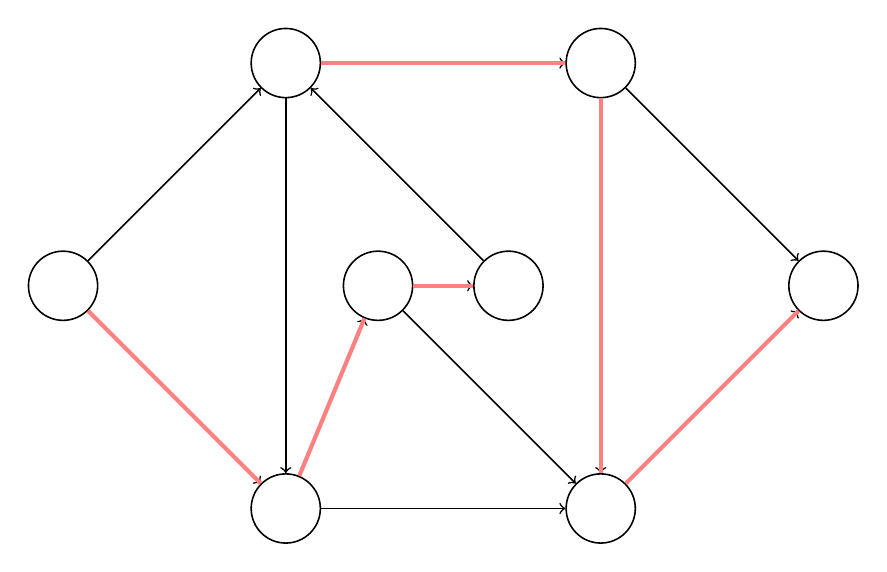
\begin{tikzpicture}[->,auto,node distance=4cm,line width=0.2mm]
  \tikzstyle{selected edge} = [draw,line width=1.5pt,-,red!50]
  \node[state] 				(A)                   	 		{};
  \node[state]         			(B) [above right of=A] 	{};
  \node[state]				(C) [below right of=A]	{};
  \node[state]				(D) [right of=C]		{};
  \node[state]				(E) [above left of=D]	{};
  \node[state]				(F) [below right of=B]	{};
  \node[state]				(G) [right of=B]		{};
  \node[state]				(I) [below right of=G]	{};

  \path 	(A) edge node {} (B);
  \path 	(A) edge node {} (C);
  \path 	(B) edge node {} (C);
  \path 	(C) edge node {} (E);
  \path 	(E) edge node {} (F);
  \path 	(F) edge node {} (B);
  \path 	(C) edge node {} (D);
  \path 	(E) edge node {} (D);
  \path 	(G) edge node {} (D);
  \path 	(G) edge node {} (I);
  \path 	(D) edge node {} (I);
  \path 	(B) edge node {} (G);

	 \draw[selected edge] (A) -- (C);
	 \draw[selected edge] (C) -- (E);
	 \draw[selected edge] (E) -- (F);
	 \draw[selected edge] (B) -- (G);
	 \draw[selected edge] (G) -- (D);
	 \draw[selected edge] (D) -- (I);
\end{tikzpicture}
\caption{Graf med Hamilton-sti.}
\end{figure}

Vi kan enkelt få til eksponentiell-tid algoritme for $HAMPATH$-problemet ved å modifisere brute-force algoritmen for $PATH$. Vi trenger bare å bekrefte at stien er en Hamilton-sti. Ingen vet om den er løselig i polynom-tid.

$HAMPATH$-problemet har en egenskap kalt \textbf{polynom verifiserbarhet}, som er viktig i forståelsen av kompleksitet. Bekrefte eksistensen av en Hamilton-sti er mye lettere enn å bestemme dens eksistens.

\theoremstyle{mytheoremstyle}
\newtheorem{ver}{Definisjon}[section]
\begin{ver}
En \textbf{verifikator} for et språk $A$ er en algoritme $\mathcal{V}$, hvor
\begin{center}
$A = \{w | \mathcal{V}$ aksepterer $\langle w,c\rangle$ for en string $c$\}.
\end{center}
Vi måler tiden til en verifikator ved lengden av $w$, så en polynom-tid verifikator kjører i polynom-tid for lengden av $w$. Språket $A$ er polynom veriferserbart hvis det har en polynom-tid verifikator.
\end{ver}

En verifikator bruker ekstra informasjon, representert ved symbolet $c$ for å verifisere at en string $w$ er medlem av $A$. Denne informasjonen er kalt \textbf{sertifikat} eller \textbf{bevis} for medlemsskap i $A$.

For $HAMPATH$-problemet er sertifikatet for en string $\langle \mathcal{G} ,s,t\rangle \in HAMPATH$ enkelt nok Hamtilonstien fra $s$ til $t$.

\theoremstyle{mytheoremstyle}
\newtheorem{np}{Definisjon}[section]
\begin{np}
NP er klassen av språk som har polynom-tid verifikatorer.
\end{np}

NP-klassen er viktig fordi den inneholder mange problemer med praktisk interesse. $HAMPATH$ er en del av NP. NP betyr nondeterministisk polynom-tid. Problemer i NP blir ofte kalt NP-problemer.

\paragraph{NTM}
Følgende er en \textbf{nondeterministisk Turing maskin (NTM)} som bestemmer $HAMPATH$-problemet i nondeterministisk polynom-tid. Vi definerer tiden til en nondeterministisk maskin til å være tiden brukt av lengste beregningsgren.

$N_1$ = på input $\langle \mathcal{G},s,t \rangle$, hvor $\mathcal{G}$ er en rettet graf med noder $s$ og $t$:
\begin{enumerate}
\item{Skriv en liste med $m$ nummer, $p_1,\dots, p_m$}, hvor $m$ er antall noder i $\mathcal{G}$. Hvert nummer i lista er nondeterministisk valgt til å være mellom 1 og $m$.
\item{Sjekke om det er repetisjoner i lista. Hvis så, avvis.}
\item{Sjekke om $s = p_1$ og $t = p_m$. Hvis en av de ikke stemmer, avvis.}
\item{For hver $i$ mellom 1 og $m-1$, sjekk om $(p_i, p_{i+1})$ er en kant i $\mathcal{G}$. Hvis ingen er, avvis. Ellers, om alle tester er blitt suksessfulle, aksepter.}
\end{enumerate}

\paragraph{Analyse} Studere hvert steg. I steg 1, nondeterministisk seleksjon er i polynom-tid. I steg 2 og 3, hver del er en enkel sjekk, så til sammen kjøres de i polynom-tid. Steg 4 kjøres også i polynom-tid. \textbf{Merk}: denne algoritmen kjører i nondeterministisk polynom-tid.

Et språk er i NP, hvis og bare hvis, det kan bestemmes av en nondeterministisk polynom-tid Turing maskin.

\subsubsection{Konvertering av polynom-tid verifikator til NTM}
\paragraph{Problem} Hvordan konvertere en polynom-tid verifikator til en ekvivalent polynom-tid NTM og vice versa. NTM simulerer verifikatoren ved å gjette sertifikatet. Verifikatoren simulerer NTM ved bruk av de aksepterende grenene som sertifikat.

\paragraph{Bevis} La $A \in NP$ og vis at $A$ bestemmes av en polynom-tid NTM $\mathcal{N}$. La $\mathcal{V}$ være polynom-tid verifikator for $A$. Anta at $\mathcal{V}$ er en TM som skjører i $n^k$ tid og konstruerer $\mathcal{N}$ som følger:

$\mathcal{N}$ = på input $w$ av lengde $n$:
\begin{enumerate}
\item{Nondeterministisk velg en string $c$ med lengde max. $n^k$.}
\item{Kjør $\mathcal{V}$ på input $\langle w,c \rangle$}.
\item{Hvis $\mathcal{V}$ aksepterer, aksepter. Ellers, avvis.}
\end{enumerate}

Og for verifikator:
$\mathcal{V}$ = på input $\langle w,c \rangle$ hvor $w$ og $c$ er stringer:
\begin{enumerate}
\item{Simuler $\mathcal{N}$ på input $w$, og behandler hvert symbol av $c$ som beskrivelse av nondeterministisk valg for hvert steg.}
\item{Hvis denne grenen av $\mathcal{N}$ sin beregning aksepterer, aksepter. Ellers, avvis.}
\end{enumerate}

\subsubsection{Problem i NP}
En \textbf{clique} i en urettet graf er en subgraf. En k-clique er en clique som inneholder $k$ noder.

 \begin{figure}[h!]
 \centering
 \scalebox{0.6}
 {
 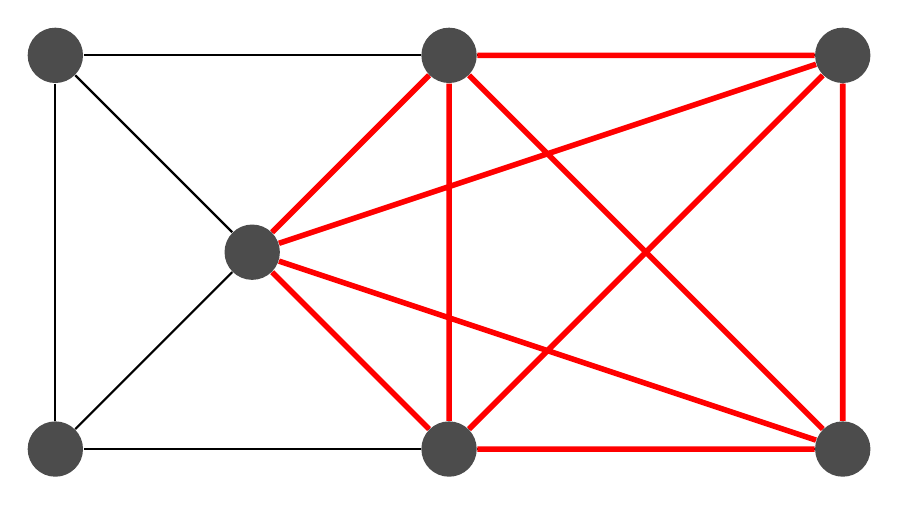
\begin{tikzpicture}[scale=5]
	 \tikzstyle{vertex}=[circle,minimum size=20pt,inner sep=0pt,fill=black!70]
	 \tikzstyle{selected vertex} = [vertex, fill=red!24]
	 \tikzstyle{selected edge} = [draw,line width=2pt,-,red!100]
	 \tikzstyle{edge} = [draw,thick,-,black]

	 \node[vertex] (v0) at (0,0) {};
	 \node[vertex] (v1) at (0,1) {};
	 \node[vertex] (v2) at (1,0) {};
	 \node[vertex] (v3) at (1,1) {};
	 \node[vertex] (v4) at (2,1) {};
	 \node[vertex] (v5) at (2,0) {};
	 \node[vertex] (v6) at (0.5,0.5) {};

	 \draw[edge] (v0) -- (v1) -- (v3) -- (v2) -- (v5) -- (v4) -- (v3) -- (v2) -- (v0); 
	 \draw[edge] (v6) -- (v0) -- (v6) -- (v1) -- (v6) -- (v2) -- (v6) -- (v3) -- (v6) -- (v4) -- (v6) -- (v5);
	 \draw[edge] (v2) -- (v4) -- (v5) -- (v3);
	 \draw[selected edge]  (v6) -- (v2) -- (v6) -- (v3) -- (v6) -- (v4) -- (v6) -- (v5) -- (v4) -- (v3) -- (v2) -- (v5) -- (v3) -- (v2) -- (v4);
 \end{tikzpicture}
 }
 \caption{5-clique}
 \end{figure}

Clique problemet avgjør om en graf inneholder en clique av en spesiell størrelse. La
\begin{center}
$CLIQUE = \{\langle \mathcal{G},k \rangle | \mathcal{G}$ er en urettet graf med en $k$-clique\}.
\end{center}

$CLIQUE$ er i NP. Er cliquen sertifikatet?

\paragraph{Bevis} Følgende er en verifikator $\mathcal{V}$ for $CLIQUE$.

$\mathcal{V}$ = på input $\langle \langle \mathcal{G},k \rangle,c\rangle$:
\begin{enumerate}
\item{Test om $c$ er i en subgraf med $k$ noder i $\mathcal{G}$.}
\item{Test om $\mathcal{G}$ inneholder alle kanter koblet med nodene i $c$.}
\item{Hvis begge er suksessfulle, aksepter. Ellers, avvis.}
\end{enumerate}

\subsection{P vs NP}
P = klassen med språk hvor medlemsskap kan bli \textit{bestemt} raskt. NP = klassen med språk hvor medlemsskap kan bli \textit{verifisert} raskt.

$HAMPATH$ og $CLIQUE$ er i NP, men de er ikke kjent i P. Selv om det er vanskelig å forestille seg, kan P og NP være ekvivalente. Men de kan \textit{ikke bevises} eksistens av et enkelt språk i NP som ikke er i P. Spørsmålet om P = NP er en av de største uløste problemer i historien.

\subsection{NP-kompletthet}
Hvis problemer i NP krever mer enn polynom-tid, så vil også et NP-komplett (NPC) problem gjøre det. NP-komplette problemer kan reduseres til problemer i NP. Et eksempel på et problem i NPC er $KNFSAT$.

\paragraph{Teorem} $KNFSAT$ er NP-komplett.
\paragraph{Bevis} Vise at $KNFSAT$ er polynom-tid reduserbart til $3SAT$. Skal da konvertere $\phi$ til $\phi'$, hvor $\phi$ er på knf og er tilfredstillbar $\Leftrightarrow$ $\phi'$ er på knf og er tilfredstillbar.

La $C_1, C_2, \dots, C_k$ være klausulene i $\phi$. Hvis $\phi$ er på $3SAT$ settes $\phi$ til å være $\phi'$. Ellers:

\begin{enumerate}
\item{For hver klausul som har én literal $(l_1)$ endres denne til $(l_1 \vee l_1 \vee l_1)$}. Denne klausulen må være sann.
\item{For hver klausul som har to literaler $(l_1 \vee l_2)$ endres denne til $(l_1 \vee l_2 \vee l_1)$. En av disse literalene må være sanne for at klausulen skal være sann.}
\item{For hver klausul som har tre literaler gjør man ingen endringer. Klausulen må være sann.}
\item{For hver klausul som har flere enn tre literaler $(l_1 \vee l_2 \vee \dots \vee l_m)$. Legger til en ny variabel $z_i$ og erstatter klausulen med $(l_1 \vee l_2 \vee z_1) \wedge (\neg z_1 \vee l_3 \vee z_2) \wedge (\neg z_2 \vee l_4 \vee z_3) \wedge \dots \wedge (\neg z_{m-3} \vee l_{m-1} \vee l_m)$. Verdien for disse må være sann.}
\end{enumerate}
\paragraph{Analyse} Konverteringen til $3SAT$ vil gå i polynom-tid. Derav er $KNFSAT \leq_{p} 3SAT$, og $KNFSAT \in NPC$.

\section{Kompleksitet i rom}
\theoremstyle{mytheoremstyle}
\newtheorem{rom}{Definisjon}[section]
\begin{rom}
La $\mathcal{M}$ være en deterministisk Turing maskin som stagnerer på alle input. Kompleksiteten i rommet til $\mathcal{M}$ er funksjonen $f : \mathcal{N} \rightarrow \mathcal{N}$, hvor $f(n)$ er maksimum antall av tape-celler som $\mathcal{M}$ scanner på hvilket som helst input av lengde $n$. Hvis kompleksiteten til rommet til $\mathcal{M}$ er $f(n)$, sier vi at $\mathcal{M}$ kjører i rom $f(n)$.

Hvis $\mathcal{M}$ er en nondeterministisk Turing maskin hvor alle grener stagnerer på alle input, definerer vi kompleksiteten i rommet $f(n)$ til å være maksimum antall tape-celler som $\mathcal{M}$ scanner på hvilken som helst gren av dens beregning for hvilken som helst input av lengde $n$.
\end{rom}

\theoremstyle{mytheoremstyle}
\newtheorem{rom2}{Definisjon}[section]
\begin{rom2}
La $f : \mathcal{N} \rightarrow \mathcal{R}^+$ være en funksjon. Kompleksiteten i rom-klassene, $SPACE (f(n))$ og $NSPACE (f(n))$, er definert slik: 

$SPACE (f(n)) = \{$L $|$ L er et språk som er bestemt av en $O(f(n))$-rom DTM\}.

$NSPACE (f(n)) = \{$L $|$ L er et språk som er bestemt av en $O(f(n))$-rom NTM\}.
\end{rom2}

\paragraph{Eksempel} $SAT$ kan bli løst med en lineær-rom algoritme. Antar at $SAT$ ikke kan løses med en polynom-tid algoritme, mye mindre med lineær-tid algoritme, fordi $SAT$ er NP-komplett. Rom ser ut til å være mer kraftfult enn tid fordi rom kan reduseres, mens tid kan ikke.
\newline
\newline
$\mathcal{M}_1$ = på input $\langle \phi \rangle$, hvor $\phi$ er en boolsk formel:
\begin{enumerate}
\item{For hver sanne tilordning til variablene $x_1, \dots, x_m$} av $\phi$:
\begin{itemize}
\item{Evaluer $\phi$ på den tilordningen.}
\end{itemize}
\item{Hvis $\phi$ noen gang blir evaluert til 1, aksepter. Ellers, avvis.}
\end{enumerate}

Maskinen $\mathcal{M}_1$ kjører i lineært-rom fordi hver interaksjon av loopen kan gjenbruke samme porsjon av tapen. Maskinen trenger bare å lagre den gjeldene sanne tilordningen, og kan bli utført med $O(m)$ rom. Antall variabler $m$ er maksimum $n$, lengden av inputen, så denne maskinen kjører i rom $O(n)$.

\subsection{Savitchs teorem}
Dette teoremet viset at deterministiske maskiner kan simulere nondeterministiske maskiner ved å bruke overraskende lite rom. For kompleksitet i tid vil en slik simulering trenge eksponentiell økning i tid. For kompleksitet i rom viser Savitch teorem at hvilken som helst NTM som bruker $f(n)$ rom kan bli konvertert til en DTM som bruker bare $f^2(n)$ rom.

\paragraph{Savitchs teorem}
For hvilken som helst funksjon $f : \mathcal{N} \rightarrow \mathcal{R}^+$, hvor $f(n) \geq n$, $NSPACE (f(n)) \subseteq SPACE (f^2(n))$.




\end{document}